\section{Seeded Sampling Controls}
\subsection{Policies and protocol}
To examine whether the initial comparison depended on deterministic sampling
alignment, we add reservoir sampling and randomized-phase uniform sampling.
The receivers, thresholds, original observations, eligibility rules, context
window, reporting epochs, and four byte caps remain unchanged. Receiver parameters
are loaded exactly from the completed pilot, not fitted again. Before reusing the
original controls, the runner verifies source/cache identity, receiver-file equality,
evaluation-source hashes, and every original packet stream's hash.

Reservoir sampling uses Algorithm R as reviewed by
\citet{vitter1985reservoir}. With raw capacity $K$, observation $i$ is stored while
$i\leq K$; subsequently a uniform integer $j\in\{0,\ldots,i-1\}$ replaces slot
$j$ when $j<K$. An unused draw is also made during the initial fill to couple
random draws across capacities without changing the marginal sampling rule.
Under ideal uniform draws, the final reservoir is a uniform sample without
replacement of $\min(K,N)$ observations. It uses bounded epoch state and does not
require the final observation count. Replacement before packet finalization is
causal because all policies deliver their packet at epoch end.

Randomized-phase uniform sampling draws an integer phase $\phi$ uniformly from
$\{0,\ldots,T-1\}$ and schedules target $j$ at offset $(jT+\phi)/K$. It retains
the first available observation at or after a target. A gap can skip several
targets but cannot cause a duplicate record; a target without a later observation
inside its epoch remains unfilled. Integer comparisons avoid timestamp-rounding
ambiguity. This is uniform sampling in time with randomized phase, not a claim
of equal inclusion probabilities for irregularly spaced observations.

Seeds 0--9 were enumerated before this comparison and all are reported. A generator
for each policy/seed/epoch is initialized from SHA-256 of those identifiers.
Budget is omitted to couple random numbers across caps. Skipping an earlier epoch
cannot shift another epoch's sequence. Budgets are correlated comparisons, and
reservoir sets across capacities need not be nested. The two policies, four caps,
and ten seeds produce 80 new arms. Capture workers receive observations and
randomization/configuration only; all capture finishes before annotation-based
decoded evaluation begins.

\subsection{Results and sampling variability}
\begin{table}[ht]
\centering\footnotesize
% Generated randomized validation comparison; seed ranges are not event confidence intervals.
\begin{tabular}{rlrrr}
\toprule
Cap & Policy & Mean MiB & PCA events: mean [range] & Context (\%) \\
\midrule
256 & Reservoir & 6.22 & 3.9 [3, 5] & 4.8 \\
256 & Random phase & 6.20 & 4.0 [3, 5] & 4.7 \\
512 & Reservoir & 12.54 & 4.6 [3, 6] & 11.7 \\
512 & Random phase & 12.49 & 4.8 [3, 6] & 11.0 \\
1024 & Reservoir & 25.15 & 5.1 [4, 7] & 23.8 \\
1024 & Random phase & 24.96 & 5.4 [4, 8] & 21.8 \\
2048 & Reservoir & 50.67 & 7.0 [5, 9] & 50.6 \\
2048 & Random phase & 50.44 & 6.7 [5, 9] & 45.9 \\
\bottomrule
\end{tabular}

\caption{Seeded validation comparisons. Actual expenditure and context are averaged
across all ten seeds. PCA counts are means and observed seed minima/maxima out of
the same 11 source-eligible events. These ranges are not confidence intervals for
new-event performance.}
\end{table}

At the 1,024-byte hourly cap, reservoir sampling retains frozen PCA evidence for
a mean of 5.1 events, with a seed range of 4--7, using 25.15 MiB on average.
Randomized phase retains a mean of 5.4, range 4--8, using 24.96 MiB. The original
adaptive arm retains 11 events using 6.30 MiB. Mean pre-event context coverage is
23.8\% for reservoir and 21.8\% for randomized phase, compared with 64.3\% for
adaptive capture. Thus the initial adaptive result remains favorable against these
two controls within the existing validation setting.

\begin{figure}[ht]
\centering
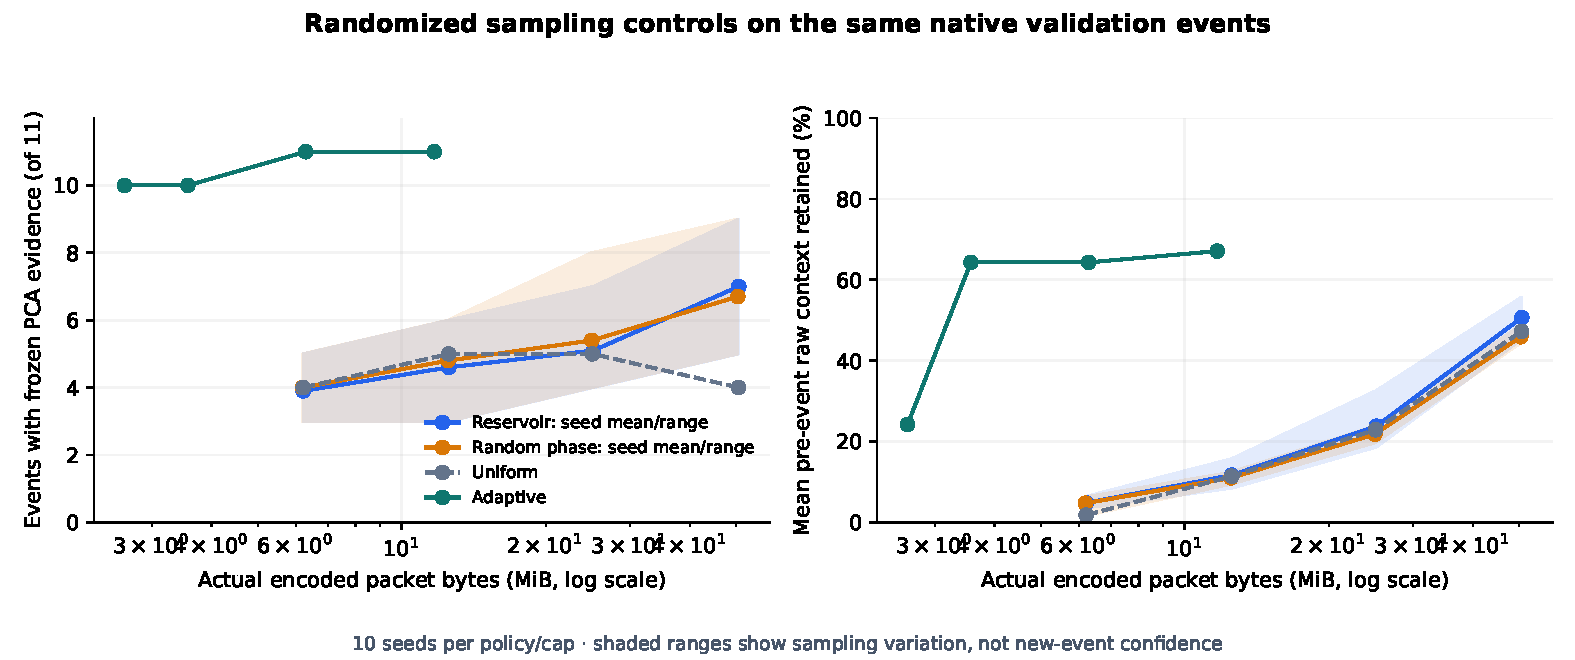
\includegraphics[width=\linewidth]{generated/randomized_tradeoff.pdf}
\caption{Means and observed seed ranges for randomized policies; original uniform
and adaptive curves are fixed controls. All methods share per-epoch byte caps,
not identical actual expenditure. Repeated seeds describe sampling variation on
this archive rather than additional independent spacecraft faults.}
\end{figure}

For the 1,024-byte streams, reservoir produces 8,016--8,125 positive normal PCA
observations and randomized phase 6,728--6,890, compared with 1,848 in the adaptive
arm. Different numbers of observations are scored, so these counts cannot be
interpreted as calibrated or comparable operational false-alarm episode rates.
The threshold-only control remains relevant: it spends 0.81 MiB and retains ten
events, exposing a cost/evidence tradeoff rather than a universal winner.

\subsection{Limits of the stronger comparison}
The ten seeds do not turn 11 events into 110 independent faults. We report every
seed and event-specific retention frequency without presenting the observed ranges
as generalization confidence intervals. The adaptive arm, including its background
sampling phase, is still deterministic. Its components have not been isolated by
this experiment. Stronger adaptive acquisition methods, component ablations,
receiver swaps, and a frozen independent-mission study remain necessary before
claims of novelty, robust diagnostic benefit, or broad superiority are warranted.
